
\chapter{A generic error structure for continuous-time dynamics.}

Real-time data commonly arrives with a variety of associated time
scales. Working with continuous time provides two key advantages
for model building.  Decisions about how to align varying time frames can be deferred
until later so that they do not drive the choice of model structure.


\section{Poisson process basics}

When describing a dynamical system we start with an arbitrary but smooth
intensity function which describes the instantenous rate of events
(e.g.- cases per day).  We are interested in producing a model for the
intensity function, written $\lambda(t)$, which describes this rate 
as a function of time.  

One obstacle we face is that we do not measure
the intensity directly, instead we measure the number of cases, $Y$,
arriving between time $s$ and time $t$.  To be exact we choose to use a  
half-open interval, $(s,t]$, to describe the period of time.  Using the
half-open interval simplifies future calculations and data preparation
by making it possible to combine intervals without calculating overlap
and to assign data unambiguously to intervals.  The complete notation
for a measurement is then $Y_{s,t,i}$ which indicates the count ($Y$),
the ends of the interval $(s,t)$, as well as an index for additioal 
covariates measured at the batch level.


\subsection{Homogenous Poisson process approximation}

In the standard application of the homogenous Poisson process, the
parameter, $m$, for the Poisson distribution can be 
calculated as the product of the fixed rate, $\lambda_i$ for batch $i$, and the
duration of time $t-s$.  This is can be thought of as a Poisson
regression where $t-s$ functions as the exposure adjustment. If $\lambda$ is 
allowed to vary by batch, this can describe a time-varying process, but at the 
cost of discontinuities.

\begin{knitrout}
\definecolor{shadecolor}{rgb}{0.969, 0.969, 0.969}\color{fgcolor}\begin{kframe}
\begin{alltt}
\hlstd{time} \hlkwb{<-} \hlnum{1}\hlopt{:}\hlnum{10}
\hlstd{rate} \hlkwb{<-} \hlkwd{seq}\hlstd{(}\hlkwc{from}\hlstd{=}\hlnum{11}\hlstd{,} \hlkwc{to}\hlstd{=}\hlnum{20}\hlstd{,} \hlkwc{length.out}\hlstd{=}\hlkwd{length}\hlstd{(time))}
\hlstd{n_per_batch} \hlkwb{<-} \hlnum{5}
\hlstd{data} \hlkwb{<-} \hlkwd{data.frame}\hlstd{(}
        \hlkwc{time} \hlstd{=} \hlkwd{rep}\hlstd{(time,n_per_batch),}
        \hlkwc{rate} \hlstd{=} \hlkwd{rep}\hlstd{(rate,n_per_batch)}
\hlstd{)}
\hlstd{data[[}\hlstr{'count'}\hlstd{]]} \hlkwb{<-} \hlkwd{rpois}\hlstd{(}\hlkwc{n}\hlstd{=}\hlkwd{nrow}\hlstd{(data),} \hlkwc{lambda}\hlstd{=data[[}\hlstr{'rate'}\hlstd{]])}
\hlstd{data} \hlkwb{<-} \hlstd{data[}\hlkwd{order}\hlstd{(data[[}\hlstr{'time'}\hlstd{]]),]}

\hlstd{f} \hlkwb{<-} \hlkwa{function}\hlstd{(}\hlkwc{lambdas}\hlstd{) \{}
        \hlstd{data[[}\hlstr{'lambda'}\hlstd{]]} \hlkwb{<-} \hlstd{lambdas[data[[}\hlstr{'time'}\hlstd{]]]}
        \hlstd{ll} \hlkwb{<-} \hlkwd{sum}\hlstd{(}\hlkwd{dpois}\hlstd{(}\hlkwc{x}\hlstd{=data[[}\hlstr{'count'}\hlstd{]],} \hlkwc{lambda}\hlstd{=data[[}\hlstr{'lambda'}\hlstd{]],} \hlkwc{log}\hlstd{=}\hlnum{TRUE}\hlstd{))}
        \hlkwd{return}\hlstd{(}\hlopt{-}\hlstd{ll)}
\hlstd{\}}

\hlstd{optzd} \hlkwb{<-} \hlkwd{optim}\hlstd{(}
        \hlkwc{par} \hlstd{=} \hlnum{12}\hlopt{:}\hlnum{21}\hlstd{,}
        \hlkwc{fn} \hlstd{= f,} \hlkwc{gr}\hlstd{=}\hlkwa{NULL}\hlstd{,}
        \hlkwc{method} \hlstd{=} \hlkwd{c}\hlstd{(}\hlstr{"L-BFGS-B"}\hlstd{),}
        \hlkwc{lower}\hlstd{=}\hlnum{10}\hlopt{^-}\hlnum{10}\hlstd{,} \hlkwc{upper}\hlstd{=}\hlnum{50}
\hlstd{)}

\hlstd{g} \hlkwb{<-} \hlkwa{function}\hlstd{(}\hlkwc{t}\hlstd{) optzd[[}\hlstr{'par'}\hlstd{]][}\hlkwd{floor}\hlstd{(t)}\hlopt{+}\hlnum{1}\hlstd{]}

\hlstd{ptzd} \hlkwb{<-} \hlkwd{data.frame}\hlstd{(}
        \hlkwc{x} \hlstd{=} \hlnum{0}\hlopt{:}\hlnum{9}\hlopt{+}\hlnum{.5}\hlstd{,}
        \hlkwc{y} \hlstd{=} \hlkwd{g}\hlstd{(}\hlnum{0}\hlopt{:}\hlnum{9}\hlopt{+}\hlnum{0.5}\hlstd{)}
\hlstd{)}

\hlkwd{library}\hlstd{(ggplot2)}
\hlstd{pl} \hlkwb{<-} \hlkwd{ggplot}\hlstd{(}
        \hlkwc{data}\hlstd{=data,}
        \hlkwd{aes}\hlstd{(}\hlkwc{x}\hlstd{=time}\hlopt{-}\hlnum{0.5}\hlstd{,} \hlkwc{y}\hlstd{=count)}
\hlstd{)} \hlopt{+} \hlkwd{geom_point}\hlstd{()} \hlopt{+}
                \hlkwd{geom_bar}\hlstd{(} \hlkwc{data}\hlstd{=ptzd,} \hlkwd{aes}\hlstd{(}\hlkwc{x}\hlstd{=x,}\hlkwc{y}\hlstd{=y),} \hlkwc{alpha}\hlstd{=}\hlnum{0.4}\hlstd{,} \hlkwc{stat}\hlstd{=}\hlstr{'identity'}\hlstd{)}
\end{alltt}
\end{kframe}
\end{knitrout}

\begin{knitrout}
\definecolor{shadecolor}{rgb}{0.969, 0.969, 0.969}\color{fgcolor}\begin{kframe}
\begin{alltt}
\hlkwd{saveRDS}\hlstd{(}\hlkwc{object}\hlstd{=pl,} \hlkwc{file}\hlstd{=}\hlkwd{file.path}\hlstd{(figure_dir,}\hlstr{'discrete-homo-poisson-process.rds'}\hlstd{))}
\end{alltt}
\end{kframe}
\end{knitrout}

\begin{knitrout}
\definecolor{shadecolor}{rgb}{0.969, 0.969, 0.969}\color{fgcolor}\begin{kframe}
\begin{alltt}
\hlstd{pl} \hlkwb{<-} \hlkwd{readRDS}\hlstd{(}\hlkwc{file}\hlstd{=}\hlkwd{file.path}\hlstd{(figure_dir,} \hlstr{'discrete-homo-poisson-process.rds'}\hlstd{))}
\hlkwd{print}\hlstd{(pl)}
\end{alltt}
\end{kframe}\begin{figure}[]

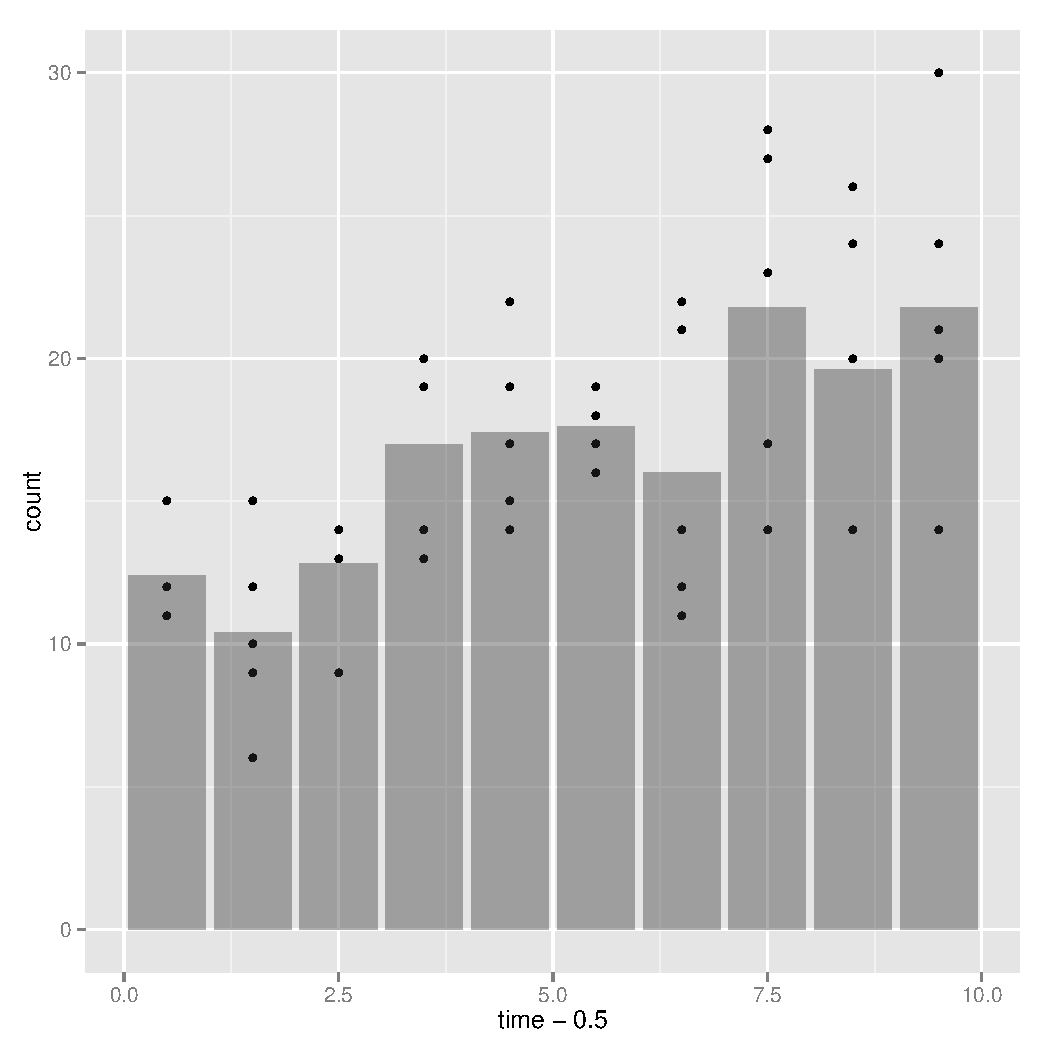
\includegraphics[width=\maxwidth]{figure/print-discrete-homo} \caption[Counts drawn from a Poisson distribution with time-varying rate]{Counts drawn from a Poisson distribution with time-varying rate.  Shaded areas describe the estimated probability mass function.  When boundaries between batches are biologically relevant this model is appropriate, but if boundaries are fluid the interpretability of the parameter at the boundary is limited.\label{fig:print-discrete-homo}}
\end{figure}


\end{knitrout}

As long as data is collected over well defined periods which match the
biological process being observed, the discontinuities are unimportant.
Sometimes, collection times vary and they may not be timed to changes in
the evolution of the biological process or the biological process may
be very dynamic as well as continuous which makes it difficult to time
data collection such that per-batch rate estimates are biologically
meaningful.  


\subsection{Inhomogenous Poisson process (IHPP)}

One way to avoid introducing the ambiguities that come with discrete
parameter batches is to use a continuous formulation of the Poisson
process which allows for a time-varying rate.  For any particular
count, $Y_{s,t,i}$, there is still a single paramter $m$, but now the
rate over the interval $(s,t]$ varies so we can no longer find the area, 
$m$, by multiplying the rate by the interval duration.  Instead we
define the intensity (or rate) function $\lambda(t)$ over the course
of the experiment.  To find the area $m_i(s,t)$ we use integration:

\begin{align}
	m_i(s,t) = \int_s^t \lambda_i(x)dx
\end{align}

Each count from a batch is still modeled as a Poisson distributed
random variable with parameter $m_i(s,t)$.  

\begin{knitrout}
\definecolor{shadecolor}{rgb}{0.969, 0.969, 0.969}\color{fgcolor}\begin{kframe}
\begin{alltt}
\hlkwd{library}\hlstd{(cruftery)}
\hlstd{data} \hlkwb{<-} \hlkwd{data.frame}\hlstd{(}
        \hlkwc{x}\hlstd{=}\hlkwd{seq}\hlstd{(}\hlkwc{from}\hlstd{=}\hlnum{0}\hlstd{,} \hlkwc{to}\hlstd{=}\hlnum{10}\hlstd{,} \hlkwc{length.out}\hlstd{=}\hlnum{10}\hlopt{^}\hlnum{3}\hlstd{),}
        \hlkwc{y}\hlstd{=}\hlkwd{gaussian_spline}\hlstd{(}\hlkwc{x}\hlstd{=}\hlkwd{seq}\hlstd{(}\hlkwc{from}\hlstd{=}\hlnum{0}\hlstd{,} \hlkwc{to}\hlstd{=}\hlnum{10}\hlstd{,} \hlkwc{length.out}\hlstd{=}\hlnum{10}\hlopt{^}\hlnum{3}\hlstd{),}
        \hlkwc{knot_points}\hlstd{=}\hlnum{2}\hlopt{:}\hlnum{8}\hlstd{,} \hlkwc{knot_weights}\hlstd{=}\hlkwd{exp}\hlstd{(}\hlkwd{rnorm}\hlstd{(}\hlnum{7}\hlstd{))}\hlopt{*}\hlnum{2}\hlopt{+}\hlkwd{c}\hlstd{(}\hlnum{0}\hlstd{,}\hlnum{2}\hlstd{,}\hlnum{2}\hlstd{,}\hlnum{2}\hlstd{,}\hlkwd{rep}\hlstd{(}\hlnum{0}\hlstd{,}\hlnum{3}\hlstd{)),} \hlkwc{knot_scale}\hlstd{=}\hlnum{0.5}\hlstd{)}
\hlstd{)}
\hlstd{shade} \hlkwb{<-} \hlstd{data[data[[}\hlstr{'x'}\hlstd{]]} \hlopt{>=} \hlnum{3} \hlopt{&} \hlstd{data[[}\hlstr{'x'}\hlstd{]]} \hlopt{<} \hlnum{5}\hlstd{,]}
\hlstd{shade} \hlkwb{<-} \hlkwd{rbind}\hlstd{(}
        \hlkwd{data.frame}\hlstd{(}\hlkwc{x}\hlstd{=}\hlnum{3}\hlstd{,}\hlkwc{y}\hlstd{=}\hlnum{0}\hlstd{),}
        \hlstd{shade,}
        \hlkwd{data.frame}\hlstd{(}\hlkwc{x}\hlstd{=}\hlnum{5}\hlstd{,}\hlkwc{y}\hlstd{=}\hlnum{0}\hlstd{)}
\hlstd{)}


\hlstd{pl} \hlkwb{<-} \hlkwd{ggplot}\hlstd{(}\hlkwc{data}\hlstd{=data,} \hlkwd{aes}\hlstd{(}\hlkwc{x}\hlstd{=x,} \hlkwc{y}\hlstd{=y))} \hlopt{+} \hlkwd{geom_line}\hlstd{()} \hlopt{+}
                        \hlkwd{geom_polygon}\hlstd{(}\hlkwc{data}\hlstd{=shade,} \hlkwd{aes}\hlstd{(}\hlkwc{x}\hlstd{=x,} \hlkwc{y}\hlstd{=y),} \hlkwc{alpha}\hlstd{=}\hlnum{0.3}\hlstd{)} \hlopt{+}
                        \hlkwd{xlab}\hlstd{(}\hlstr{'Time (days)'}\hlstd{)} \hlopt{+} \hlkwd{ylab}\hlstd{(}\hlstr{'Intensity (Cases per day)'}\hlstd{)} \hlopt{+}
                        \hlkwd{annotate}\hlstd{(}\hlstr{"text"}\hlstd{,} \hlkwc{x}\hlstd{=}\hlnum{3}\hlstd{,} \hlkwc{y}\hlstd{=}\hlopt{-}\hlnum{.2}\hlstd{,} \hlkwc{label}\hlstd{=}\hlstr{"s"}\hlstd{)} \hlopt{+}
                        \hlkwd{annotate}\hlstd{(}\hlstr{"text"}\hlstd{,} \hlkwc{x}\hlstd{=}\hlnum{5}\hlstd{,} \hlkwc{y}\hlstd{=}\hlopt{-}\hlnum{.2}\hlstd{,} \hlkwc{label}\hlstd{=}\hlstr{"t"}\hlstd{)} \hlopt{+}
                        \hlkwd{annotate}\hlstd{(}\hlstr{"text"}\hlstd{,} \hlkwc{x}\hlstd{=}\hlnum{4}\hlstd{,} \hlkwc{y}\hlstd{=} \hlnum{.8}\hlstd{,} \hlkwc{label}\hlstd{=}
                                \hlstr{"m(s,t)==integral(lambda(x)*dx,s,t)"}\hlstd{,} \hlkwc{parse}\hlstd{=}\hlnum{TRUE}\hlstd{)}
\end{alltt}
\end{kframe}
\end{knitrout}

\begin{knitrout}
\definecolor{shadecolor}{rgb}{0.969, 0.969, 0.969}\color{fgcolor}\begin{kframe}
\begin{alltt}
\hlkwd{saveRDS}\hlstd{(}\hlkwc{object}\hlstd{=pl,} \hlkwc{file}\hlstd{=}\hlkwd{file.path}\hlstd{(figure_dir,}\hlstr{'cont-inhomo-poisson-process.rds'}\hlstd{))}
\end{alltt}
\end{kframe}
\end{knitrout}

\begin{knitrout}
\definecolor{shadecolor}{rgb}{0.969, 0.969, 0.969}\color{fgcolor}\begin{kframe}
\begin{alltt}
\hlstd{pl} \hlkwb{<-} \hlkwd{readRDS}\hlstd{(}\hlkwc{file}\hlstd{=}\hlkwd{file.path}\hlstd{(figure_dir,} \hlstr{'cont-inhomo-poisson-process.rds'}\hlstd{))}
\hlkwd{print}\hlstd{(pl)}
\end{alltt}
\end{kframe}\begin{figure}[]

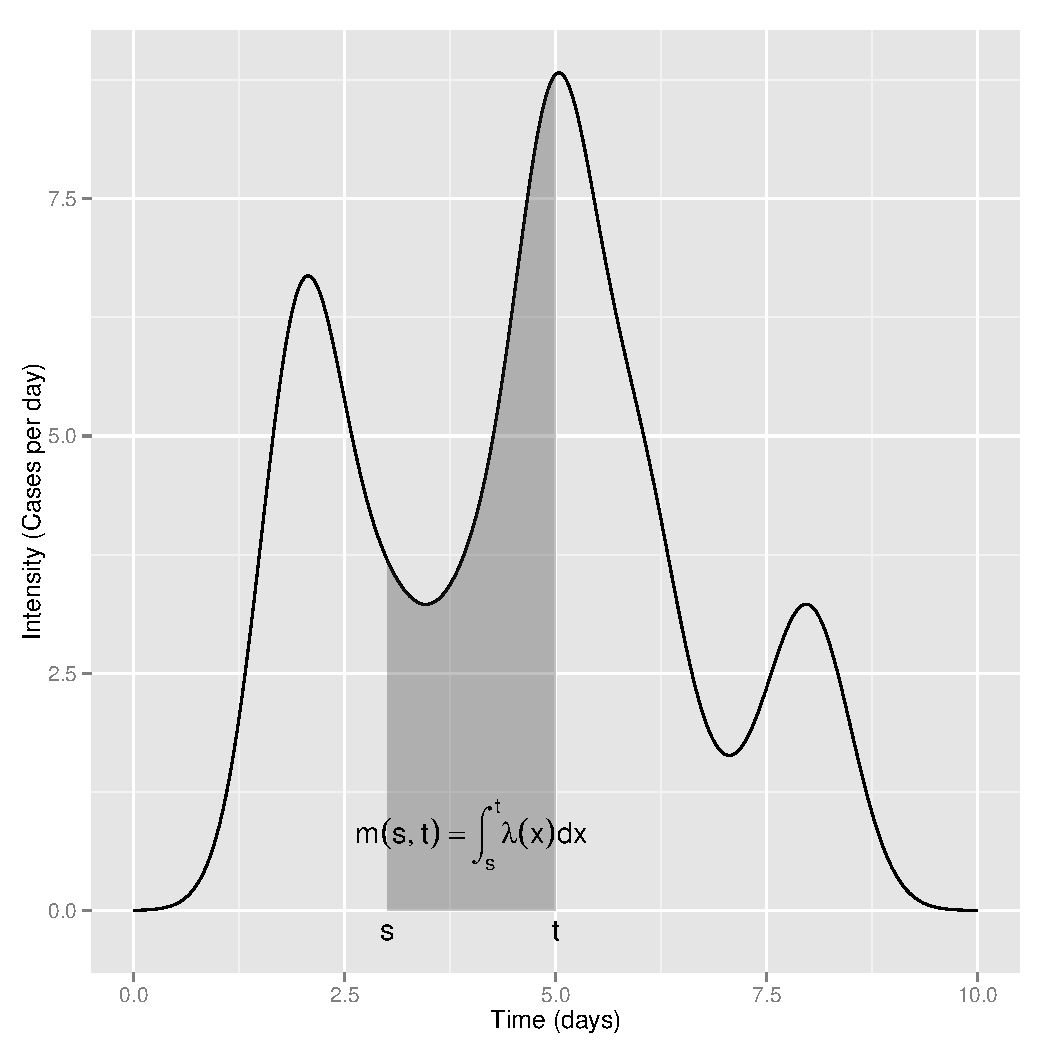
\includegraphics[width=\maxwidth]{figure/print-cont-inhomo} \caption[Counts drawn from a Poisson distribution with time-varying rate]{Counts drawn from a Poisson distribution with time-varying rate.  The curve is the intensity function in units of cases per day, which is integrated to give the Poisson distribution parameter.\label{fig:print-cont-inhomo}}
\end{figure}


\end{knitrout}

The inhomogenous poisson process makes an effective bridge between a
process conceptualized as continuous and real data collected on varying
time scales in a discrete fashion.  The focus of any further effort
can be on the function $\lambda(t)$ which is the rate of cases per
unit time.  The remaining difficulty is choosing a form of $\lambda(t)$
which is easy to integrate and allows us to apply the usual ameneties
of statistics---design matrices and linear models.

\section{Poisson process implementation}\label{sec:ihpp-implementation}

The two conditions on $\lambda(t)$ are that it should be easy to
integrate and that is should be amenable to further modeling.  For
this second reason, we choose to use a semiparameteric radial spline.
We spread $K$ knot points over the time period covered by the data
and use the normal distribution as a basis function.  The basis set is
then the set of normals centered on each knot point.  The function
$\lambda(t)$ then becomes a weighted sum of $K$ normals.

\begin{align}
\lambda(x) &= \sum_{k=1}^K \beta_k \frac{1}{\sqrt{2\pi}\sigma^2} \exp(\frac{1}{2\sigma^2}\left(x-\mu_k\right)^2)
\end{align}

This formulation allows us to further model the weights $\beta_k$ to
describe the effects relevant to a specific portion of time without
introducing discontinuities in the intensity function while still making
the function very flexible.  Formulating the intensity function as a sum
of normal densities also makes analytical integration possible as long
as the function has a known $CDF$.  Abusing notation slightly, the 
calculation of $m(s,t)$ becomes:

\begin{align}
m(s,t) &= \int_s^t \sum_{k=1}^K \beta_k PDF_N(x,\mu_k,\sigma^2) dx \\
			 &= \sum_{k=1}^K \beta_k \left(CDF_N(t,\mu_k,\sigma^2) - CDF_N(s,\mu_k,\sigma^2) \right)
\end{align}

Since calculations of many $CDF$'s, including the normal, are
efficiently coded in many libraries this is a generic strategy for
applying the IHPP to a variety of problems.  
















